% =============================================================
%  Thesis progress update, Transavia & Accenture
%  Author: Noah Bos
%  Date: 2026-05-27
%  Style: Accenture-inspired (purple #A100FF, sans-serif, clean)
%  Compile: pdflatex thesis_update_2026-05-27.tex   (run twice)
% =============================================================

\documentclass[aspectratio=169,11pt]{beamer}

% ---- Packages ----
\usepackage[T1]{fontenc}
\usepackage[utf8]{inputenc}
\usepackage{lmodern}
\usepackage{helvet}
\renewcommand{\familydefault}{\sfdefault}
\usepackage{xcolor}
\usepackage{tikz}
\usepackage{booktabs}
\usepackage{array}
\usepackage{tabularx}
\usepackage{calc}

% ---- Accenture palette ----
\definecolor{accpurple}{HTML}{A100FF}      % signature purple
\definecolor{accdark}{HTML}{1F1F1F}        % near-black text
\definecolor{accgray}{HTML}{6B6B6B}        % secondary text
\definecolor{accbg}{HTML}{F5F2FA}          % subtle purple wash
\definecolor{accaccent}{HTML}{460073}      % deep purple accent
\definecolor{accgreen}{HTML}{1AAF54}       % callout: good
\definecolor{accred}{HTML}{D6336C}         % callout: risk

% ---- Beamer setup: clean, no nav bars, frame number only ----
\setbeamertemplate{navigation symbols}{}
\setbeamertemplate{footline}{%
  \leavevmode%
  \hbox{%
    \begin{beamercolorbox}[wd=\paperwidth, ht=2.5ex, dp=1ex, right, rightskip=1.2em]{}%
      \color{accpurple}\scriptsize\insertframenumber{}\,/\,\inserttotalframenumber
    \end{beamercolorbox}}\vskip0pt%
}

\setbeamercolor{frametitle}{fg=accdark, bg=white}
\setbeamercolor{title}{fg=accdark}
\setbeamercolor{normal text}{fg=accdark, bg=white}
\setbeamercolor{itemize item}{fg=accpurple}
\setbeamercolor{itemize subitem}{fg=accpurple}
\setbeamercolor{itemize subsubitem}{fg=accpurple}
\setbeamercolor{enumerate item}{fg=accpurple}
\setbeamercolor{block title}{fg=white, bg=accpurple}
\setbeamercolor{block body}{fg=accdark, bg=accbg}
\setbeamercolor{alerted text}{fg=accred}

\setbeamerfont{frametitle}{size=\large, series=\bfseries}
\setbeamerfont{title}{size=\LARGE, series=\bfseries}
\setbeamerfont{subtitle}{size=\normalsize, series=\mdseries}

% Frame title with purple underline
\setbeamertemplate{frametitle}{%
  \vspace{0.8em}%
  \hspace{0.6em}\insertframetitle\\[-0.2em]%
  \hspace{0.6em}\textcolor{accpurple}{\rule{2.5em}{2pt}}\vspace{0.4em}%
}

\setbeamertemplate{itemize item}{\raisebox{0.3ex}{\scalebox{0.7}{\textcolor{accpurple}{$\blacksquare$}}}}
\setbeamertemplate{itemize subitem}{\raisebox{0.3ex}{\scalebox{0.6}{\textcolor{accpurple}{$\blacktriangleright$}}}}

% Custom title page
\defbeamertemplate*{title page}{accenture}{%
  \begin{tikzpicture}[remember picture, overlay]
    \fill[accpurple] (current page.north west) rectangle ([yshift=-1.3cm]current page.north east);
    \fill[accaccent] ([yshift=-1.3cm]current page.north west) rectangle ([yshift=-1.45cm]current page.north east);
  \end{tikzpicture}%
  \vspace{2.8cm}
  \begin{flushleft}
    \hspace{0.8em}{\color{accpurple}\rule{3em}{3pt}}\\[0.6em]
    \hspace{0.8em}{\usebeamerfont{title}\inserttitle}\\[0.4em]
    \hspace{0.8em}{\color{accgray}\usebeamerfont{subtitle}\insertsubtitle}\\[1.6em]
    \hspace{0.8em}{\color{accdark}\small\insertauthor}\\[0.2em]
    \hspace{0.8em}{\color{accgray}\footnotesize\insertdate}
  \end{flushleft}
}

% Section divider command
\newcommand{\sectiondivider}[2]{%
  \begin{frame}[plain, noframenumbering]
    \begin{tikzpicture}[remember picture, overlay]
      \fill[accpurple] (current page.south west) rectangle (current page.north east);
    \end{tikzpicture}
    \vfill
    \begin{center}
      \color{white}{\fontsize{12}{14}\selectfont\textbf{PART #1}}\\[0.6em]
      \color{white}{\fontsize{28}{32}\selectfont\textbf{#2}}\\[0.6em]
      \color{white}{\rule{4em}{2pt}}
    \end{center}
    \vfill
  \end{frame}
}

% Inline coloured chip
\newcommand{\chip}[2]{\tikz[baseline=(c.base)]{\node[fill=#1!15, draw=#1, line width=0.4pt, rounded corners=2pt, inner sep=2pt, text=#1, font=\scriptsize\bfseries] (c) {#2};}}
\newcommand{\good}[1]{\chip{accgreen}{#1}}
\newcommand{\warn}[1]{\chip{accred}{#1}}
\newcommand{\info}[1]{\chip{accpurple}{#1}}

% =============================================================
%  TITLE
% =============================================================
\title{Surrogate-based stability of Pega ADM explanations}
\subtitle{Thesis progress + L5B15 Health Check findings}
\author{Noah Bos \textbar{} Accenture \textbar{} Leiden University thesis}
\date{27 May 2026}

\begin{document}

% ---------- Title ----------
\begin{frame}[plain, noframenumbering]
  \titlepage
\end{frame}

% ---------- Agenda ----------
\begin{frame}{Agenda}
  \vspace{0.3em}
  \begin{enumerate}
    \setlength\itemsep{0.7em}
    \item \textbf{Where the thesis stands}, stability of feature attributions
    \item \textbf{Bonus: L5B15 Health Check findings}, what Pega's own tool reveals
    \item \textbf{Forward look}, predictors that could lift luggage CTR
    \item \textbf{Next steps \& open questions}
  \end{enumerate}
  \vspace{1em}
  \begin{block}{Framing}
    Sections 1 \& 4 are the academic deliverable.\\
    Sections 2 \& 3 are \emph{hypotheses surfaced by the Health Check review}, directions to validate, not actions to take tomorrow.
  \end{block}
\end{frame}

% =============================================================
%  PART 1: THESIS PROGRESS
% =============================================================
\sectiondivider{1}{Where the thesis stands}

\begin{frame}{Three research questions}
  \begin{tabularx}{\linewidth}{@{}p{1.2em}X@{}}
    \textcolor{accpurple}{\textbf{RQ1}} & How accurately do SHAP, LIME and Decision Tree surrogates approximate the Pega black-box propensity model? \\[0.7em]
    \textcolor{accpurple}{\textbf{RQ2}} & How stable are feature attribution rankings across temporal splits and route subgroups? \\[0.7em]
    \textcolor{accpurple}{\textbf{RQ3}} & Does observed instability reflect data drift ($\delta_d$), model churn ($\delta_m$), or explainer sensitivity ($\delta_e$)? \\
  \end{tabularx}
  \vspace{0.5em}
  \begin{block}{Scope}
    Luggage upsell, Email/Outbound channel. Primary variant: \textbf{L5B15}. Replicated on CLUG, BookingDotCom, Cartrawler.
  \end{block}
\end{frame}

\begin{frame}{Why a CatBoost surrogate, and how well it works}
  Pega ADM uses Naive Bayes internally. We train CatBoost \emph{on} Pega's output propensities.
  \vspace{0.4em}
  \begin{itemize}
    \item \textbf{TreeSHAP requires a tree model}, KernelSHAP on NB would $\sim$100$\times$ compute and stack its own error
    \item \textbf{Fidelity over mimicry}, flexible surrogate reproduces NB's mapping better than one constrained by conditional independence
    \item \textbf{Native categorical + missing handling}, no encoding choices as confounds
  \end{itemize}
  \vspace{0.4em}
  \footnotesize
  \begin{tabular}{@{}l r r r r@{}}
    \toprule
    \textbf{Variant}      & \textbf{R$^2$} & \textbf{Spearman $\rho$} & \textbf{RMSE} & \textbf{n} \\
    \midrule
    L5B15                 & 0.927          & 0.933                    & 0.0026        & 31{,}709 \\
    CLUG                  & 0.954          & 0.920                    & 0.0026        & 16{,}984 \\
    BookingDotCom         & 0.793          & 0.949                    & 0.0002        & 19{,}866 \\
    Cartrawler            & 0.912          & 0.615                    & 0.0005        & 20{,}645 \\
    \bottomrule
  \end{tabular}
  \vspace{0.3em}
  \normalsize \info{High fidelity on three of four variants. Cartrawler's low $\rho$ flags propensity-rank degradation despite good R$^2$.}
\end{frame}

\begin{frame}{Instability decomposition (RQ3) in plain language}
  We decompose how much each \textbf{ranking} changes between two splits into three sources:
  \vspace{0.6em}
  \begin{center}
    \begin{tabular}{r l}
      \textbf{DT instability}    & $=$ \ data drift \ $+$\ model churn \ $+$\ explainer gap \\[0.4em]
      \textbf{SHAP instability}  & $\approx$ \ data drift \ $+$\ model churn  \\[0.4em]
      \textbf{Explainer gap}     & $=$ \ DT instability \ $-$\ SHAP instability \\
    \end{tabular}
  \end{center}
  \vspace{0.8em}
  \begin{columns}[T,onlytextwidth]
    \column{0.32\linewidth}
    \textbf{Data drift}\\
    KS statistic on the propensity score distribution (bin-free, non-parametric).
    \column{0.32\linewidth}
    \textbf{Model churn}\\
    Jaccard overlap on the set of \texttt{modelVersion} IDs active in each split (low overlap $=$ high churn).
    \column{0.32\linewidth}
    \textbf{Explainer gap}\\
    What DT picks up that SHAP does not, i.e.\ sensitivity of the explanation method itself.
  \end{columns}
\end{frame}

\begin{frame}{Evaluation design}
  Each split is a pair of sub-populations evaluated on the same surrogate.
  \vspace{0.3em}
  \begin{itemize}
    \item \textbf{Temporal split}, early vs late window within each variant
    \item \textbf{Route subgroups}, top 4 routes by volume (e.g.\ ORY$\to$NCE, ORY$\to$OPO, NCE$\to$ORY, TLS$\to$ORY)
    \item \textbf{Culture / language split}, fr-FR vs nl-NL bookings
    \item \textbf{Replication}, L5B15 $\rightarrow$ CLUG, BookingDotCom, Cartrawler
  \end{itemize}
  \vspace{0.7em}
  \begin{block}{Why same-window splits are useful}
    Route and culture splits share a time window, so the active model snapshots are essentially the same: $\delta_m \approx 0$ and $\delta_d$ stays small. Any remaining instability is mostly $\delta_e$.\\[0.3em]
    A within-route DT bootstrap ($N=10$ seeds) gives the noise floor for DT ranking variability, so we can tell ``real'' between-route disagreement from fitting noise.
  \end{block}
\end{frame}

\begin{frame}{Stability results: L5B15, by split}
  Spearman $\rho$ between top-feature rankings (closer to 1 = more stable):
  \vspace{0.3em}
  \footnotesize
  \begin{tabular}{@{}l r r r@{}}
    \toprule
    \textbf{Split}                       & \textbf{DT $\rho$} & \textbf{LIME $\rho$} & \textbf{SHAP $\rho$} \\
    \midrule
    Temporal (early vs late)             & 0.855              & 0.989                & 0.996 \\
    Route: NCE$\to$ORY vs TLS$\to$ORY    & 0.817              & 0.992                & 0.987 \\
    Route: ORY$\to$NCE vs ORY$\to$OPO    & \warn{0.510}       & 0.986                & 0.994 \\
    Route: ORY$\to$OPO vs NCE$\to$ORY    & \warn{0.584}       & 0.858                & 0.990 \\
    Culture: fr-FR vs nl-NL              & \warn{0.667}       & 0.949                & 0.958 \\
    \bottomrule
  \end{tabular}

  \vspace{0.5em}
  {\scriptsize\textcolor{accgray}{Red highlight: DT $\rho < 0.7$, i.e.\ rankings disagree on more than 30\% of pairs.}}

  \vspace{0.4em}
  \normalsize
  \begin{block}{Pattern}
    \textbf{SHAP and LIME are very stable} ($\rho > 0.95$ almost everywhere). \textbf{DT rankings collapse} on certain route and language splits ($\rho$ down to 0.51), well below the within-route DT bootstrap noise floor (mean $\rho \approx 0.83$ across 10 seeds), so the disagreement is real, not a fluke of how the tree was fit.
  \end{block}
\end{frame}

\begin{frame}{Instability decomposition: where does it come from?}
  \vspace{-0.2em}
  \footnotesize
  \begin{tabular}{@{}l c c c l@{}}
    \toprule
    \textbf{Split}                  & \textbf{Data drift} & \textbf{Model churn} & \textbf{Explainer gap} & \textbf{Dominant} \\
                                    & \textbf{(KS)}       & \textbf{($J_v$)}     &                        &  \\
    \midrule
    Temporal (early vs late)        & 0.36                & 0.00                 & 0.141                  & external shift \\
    ORY$\to$NCE vs ORY$\to$OPO      & 0.10                & 0.48                 & 0.484                  & \warn{explainer gap} \\
    ORY$\to$OPO vs NCE$\to$ORY      & 0.09                & 0.55                 & 0.406                  & \warn{explainer gap} \\
    NCE$\to$ORY vs TLS$\to$ORY      & 0.09                & 0.52                 & 0.171                  & \warn{explainer gap} \\
    fr-FR vs nl-NL                  & 0.08                & 0.59                 & 0.291                  & \warn{explainer gap} \\
    \bottomrule
  \end{tabular}

  \vspace{0.4em}
  {\scriptsize\textcolor{accgray}{KS in $[0,1]$; significant drift if $\geq 0.10$. $J_v$ is Jaccard overlap of active \texttt{modelVersion} sets; \emph{higher} $=$ \emph{more stable}; significant churn if $J_v \leq 0.10$. Same-window splits sit near $J_v \approx 0.5$ by design, since Pega's online NB issues a fresh \texttt{modelVersion} UUID on every micro-update.}}

  \vspace{0.3em}
  \normalsize
  \begin{block}{Headline finding (RQ3)}
    \footnotesize
    On route and culture subgroups, neither the input data nor the active model versions change much, yet DT's top-feature list looks very different across them. SHAP rankings stay almost identical on the same splits, so the difference comes from the explanation method itself, not from the model. \textbf{DT can disagree with itself across populations even when the underlying model has not changed.}
  \end{block}
\end{frame}

\begin{frame}{What SHAP says are the most important features}
  Top 10 L5B15 features by mean absolute SHAP value, from the CatBoost surrogate:
  \begin{center}
    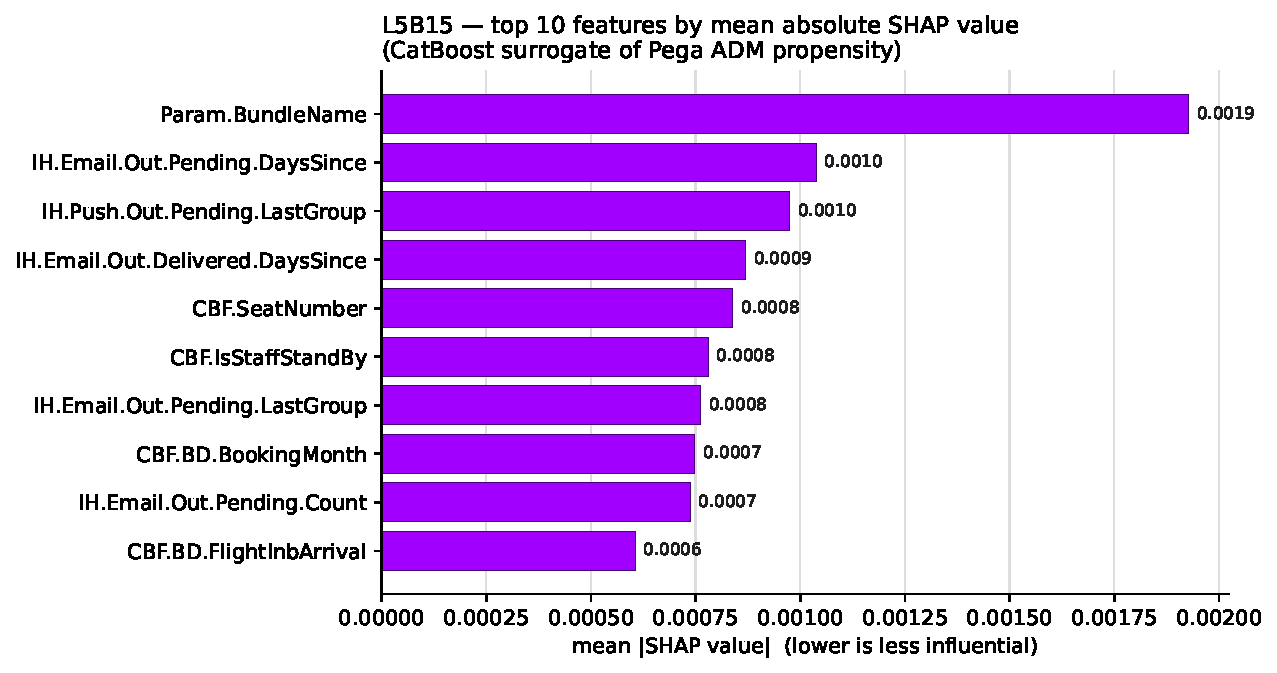
\includegraphics[width=0.94\linewidth]{figures/shap_top10_l5b15.pdf}
  \end{center}
  \vspace{-0.5em}
  \footnotesize
  \begin{block}{Why this matters}
    Eight of these ten features also appear in Pega's own top-10 by univariate AUC (next sections). The two views \emph{agree} on what drives the model, an independent confirmation of RQ1 fidelity. Differences (\texttt{CBF.SeatNumber}, \texttt{CBF.BD.FlightInbArrival}) reflect interaction effects that NB cannot capture but the surrogate can.
  \end{block}
\end{frame}

% =============================================================
%  PART 2: L5B15 HEALTH CHECK FINDINGS
% =============================================================
\sectiondivider{2}{L5B15 Health Check findings}

\begin{frame}{The Pega ADM Health Check}
  \begin{itemize}
    \item Pega's official \texttt{pdstools} tool, run on the same Datamart export this thesis uses
    \item Generic ADM overview \emph{plus} per-model deep-dives
    \item I ran it specifically against \textbf{Sales / Luggage / L5B15 / L5B15\_EM\_T01}
    \item AUC = \textbf{76.56}, responses = 2.86\,M, positives = 25{,}766 \quad \info{healthy model}
  \end{itemize}
  \vspace{0.7em}
  \begin{block}{Why this matters here}
    The Health Check views the model through Pega's own lens (univariate NB performance). Comparing it side-by-side with our surrogate's SHAP/LIME/DT importances is a direct external sanity check on RQ1 and a free source of operational insights.
  \end{block}
\end{frame}

\begin{frame}{Where L5B15 sits in the wider ADM picture}
  \begin{center}
    \vspace{0.6em}
    {\fontsize{40}{44}\selectfont\color{accpurple}\textbf{Only 36\%}}\\[0.5em]
    {\large of the 944 ADM models in the snapshot are \emph{mature and useful}.}\\[0.4em]
    \footnotesize\textcolor{accgray}{(mature = $\geq 200$ positives and AUC $\geq 0.52$)}
  \end{center}
  \vspace{1.0em}
  \footnotesize
  \begin{itemize}
    \item Email / Outbound channel: 959K positives, positive-response rate 1.63\%, average AUC 69.1
    \item Luggage group: 70 models (L5B15, L5B20, CLUG, ...)
    \item 220 models have never been used or never received a positive, dead weight in the system
  \end{itemize}
\end{frame}

\begin{frame}{L5B15: what the NB model actually uses}
  Of 220+ predictors in the pool, only \textbf{24 are Active} in the NB model.\\
  Top 10 by univariate AUC (Pega's own measure, from Predictor Overview table):
  \vspace{0.4em}
  \footnotesize
  \begin{tabular}{@{}r l r l@{}}
    \toprule
    \# & \textbf{Predictor} & \textbf{AUC} & \textbf{Note} \\
    \midrule
    1 & \texttt{Param.BundleName}                                       & 74.28 & action-label proxy \warn{verify} \\
    2 & \texttt{CustBookedFlight.BookingData.BookingMonth}              & 72.50 & seasonality \warn{verify} \\
    3 & \texttt{IH.Email.Out.Pending.pxLastOutcomeTime.DaysSince}       & 67.42 & IH recency \\
    4 & \texttt{IH.Email.Out.Pending.pyHistoricalOutcomeCount}          & 66.21 & IH volume \\
    5 & \texttt{CustBookedFlight.IsStaffStandBy}                        & 66.12 & \warn{data-gap proxy} \\
    6 & \texttt{IH.Push.Out.Pending.pyHistoricalOutcomeCount}           & 65.63 & cross-channel \\
    7 & \texttt{IH.Push.Out.Pending.pxLastOutcomeTime.DaysSince}        & 64.68 & \\
    8 & \texttt{IH.Email.Out.Pending.pxLastGroupID}                     & 64.67 & last-group context \\
    9 & \texttt{IH.Push.Out.Pending.pxLastGroupID}                      & 64.24 & \\
    10 & \texttt{IH.Email.Out.Delivered.pxLastGroupID}                  & 63.98 & \\
    \bottomrule
  \end{tabular}

  \vspace{0.4em}
  \info{Mostly a recency/fatigue machine; customer profile barely contributes.}\\[0.2em]
  {\scriptsize\textcolor{accgray}{Pega marks predictors \emph{Inactive} when their correlation with another active predictor exceeds a tunable threshold (default $\sim 0.8$) or when univariate AUC is too low. A sensitivity sweep on this cutoff is on the further-work list.}}
\end{frame}

\begin{frame}{Three anomalies worth flagging}
  \scriptsize
  \begin{tabular}{@{}p{0.18\linewidth} p{0.20\linewidth} p{0.55\linewidth}@{}}
    \toprule
    \textbf{Predictor} & \textbf{What we expected} & \textbf{What the data shows} \\
    \midrule
    \texttt{Param.\linebreak BundleName} (AUC 74)
      & The action label itself, i.e.\ trivial.
      & It is the broader email context: \emph{BookingConfirmation, InternetCheckIn, Pre\_Departure\_Outbound, AncillaryRecommender, Luggage, \ldots} The \emph{Luggage} bundle alone has positives-lift $+261\%$, driving the high AUC. Legitimate signal, but near-tautological (``show luggage in luggage-themed emails''). \\[0.4em]
    \texttt{IsStaff\-StandBy} (AUC 66)
      & A staff flag, possibly a label leak.
      & \textbf{Almost no records are actually true} (52 out of 3.15M). The high AUC comes from the \textbf{MISSING vs false} split: MISSING records ($37\%$ of pop.) convert at $-86\%$ vs base, populated records ($63\%$) at $+50\%$. The flag is really a \emph{data-completeness proxy}, not a staff indicator. \\[0.4em]
    \texttt{Booking\-Month} (AUC 72.5)
      & Calendar month, seasonality.
      & Bins read \texttt{<1.02, [1.02,2.02), [2.02,3.02), \ldots, $\geq$5.02}. Looks like \emph{months until departure} (or since booking), not a calendar month. Pattern is U-shaped: extremes convert best. Semantics need confirmation. \\
    \bottomrule
  \end{tabular}

  \vspace{0.6em}
  \footnotesize
  \textbf{All three need a one-question check with the Transavia/Pega team} before any are accepted as causal signal.
\end{frame}

\begin{frame}{The clearest business signal: message fatigue}
  \texttt{IH.Email.Out.Pending.pxLastGroupID}, bin lifts vs base rate:
  \vspace{0.5em}
  \footnotesize
  \begin{tabular}{@{}l r r@{}}
    \toprule
    \textbf{Last-group bin}     & \textbf{Lift}    & \textbf{Interpretation} \\
    \midrule
    Promotions                  & \good{+125\%}     & cold customers respond best \\
    ThirdParty                  & +40\%             & \\
    FAQs                        & $-$11\%           & \\
    BundleParent                & $-$40\%           & \\
    \textbf{Luggage}            & \warn{$-$50\%}    & recently shown luggage $\rightarrow$ \textbf{half} the CTR \\
    \bottomrule
  \end{tabular}
  \vspace{0.6em}
  \normalsize
  \begin{block}{Operational implication}
    A customer recently exposed to a luggage offer is roughly half as likely to engage with another one. Cadence / suppression rules tuned to this can raise effective CTR \emph{without changing the model}.
  \end{block}
\end{frame}

\begin{frame}{Signals that could lift CTR but are currently inaccessible}
  Today the L5B15 model is mostly a \emph{recency / fatigue machine}. Click-through prediction could likely be improved by stronger customer-level signals. Two complementary paths:
  \vspace{0.3em}
  \begin{itemize}
    \item \textbf{Cheaper}, predictors that are already configured in the model but stay inactive because the upstream data isn't flowing in. Fix the data pipeline, no feature-engineering needed.
    \item \textbf{Heavier}, customer or route-level features that would need to be designed (e.g.\ customer-segment clustering, route clusters, trip-purpose composites). Future-work track.
  \end{itemize}
  \vspace{0.4em}
  \footnotesize
  \begin{tabular}{@{}l r l@{}}
    \toprule
    \textbf{Predictor family (already configured)}                     & \textbf{Missing \%} & \textbf{Status today} \\
    \midrule
    \texttt{Customer.CustomerKPIs.*CountTotal} (per-product history)  & 75--77\%            & inactive, would personalise \\
    \texttt{IH.Push.Outbound.Received.*}                              & 90\%                & inactive \\
    \texttt{IH.Email.Outbound.Rejected.*}                             & 87\%                & inactive \\
    \texttt{IH.Email.Inbound.Rejected.*}                              & 85\%                & inactive \\
    \texttt{IH.Email.Inbound.Clicked.*}                               & 93\%                & some active despite gap \\
    \bottomrule
  \end{tabular}
\end{frame}

\begin{frame}{Bridging back to the thesis (RQ3)}
  \begin{block}{The two stories are the same story}
    The instability the thesis measures partly traces back to:
    \begin{itemize}
      \item predictors with very high missingness $\rightarrow$ unstable contributions across temporal splits (drives $\delta_d$; KS = 0.36 on L5B15 temporal)
      \item NB leaning on a small set of correlated IH counters $\rightarrow$ DT rankings collapse on route splits ($\rho$ as low as 0.51)
    \end{itemize}
    Fixing the upstream sourcing for the missing customer-history fields would reduce academic instability \emph{and} could meaningfully increase CTR.
  \end{block}
\end{frame}

% =============================================================
%  PART 3: FORWARD-LOOKING CTR LIFT
% =============================================================
\sectiondivider{3}{Forward look: lifting luggage CTR}

\begin{frame}{Three priority directions, anchored in the evidence}
  \footnotesize
  \begin{tabular}{@{}r p{0.40\linewidth} p{0.44\linewidth}@{}}
    \toprule
    \# & \textbf{Proposed lever} & \textbf{Why now (evidence)} \\
    \midrule
    1 & \textbf{Fix per-product purchase history data} (\texttt{CustomerKPIs.*}) & 75\%+ missing today; most personalisation features are blind. Unblocks a whole family of predictors. \\[0.5em]
    2 & \textbf{Cadence / suppression on recent luggage exposure} & Recent-luggage bin shows $-50\%$ lift; check current arbitration. Quick operational win, no model retrain. \\[0.5em]
    3 & \textbf{Validate the three predictor anomalies with the Transavia/Pega team} & \texttt{BundleName}, \texttt{IsStaffStandBy}, \texttt{BookingMonth}: all need a semantic check before they're trusted as causal signal. \\
    \bottomrule
  \end{tabular}
  \vspace{0.6em}
  \normalsize
  \begin{block}{Further directions for future investigation}
    \footnotesize Customer-segment clustering for personalisation \textbar{} \,
    route-cluster features (beach / city / ski / business) \textbar{} \,
    trip-purpose composite (duration $\times$ destination $\times$ children $\times$ weekday) \textbar{} \,
    cross-channel fatigue score \textbar{} \,
    sensitivity sweep on Pega's predictor-correlation cutoff.
  \end{block}
\end{frame}

\begin{frame}{Where the secondary work meets the primary work}
  \begin{block}{Two reasons the CatBoost surrogate ($R^2 \approx 0.92$) outperforms the headline NB AUC of 76}
    \begin{enumerate}
      \item NB cannot capture predictor \emph{interactions}; the surrogate can.
      \item NB's binning collapses high-cardinality categoricals; the surrogate handles them natively.
    \end{enumerate}
  \end{block}
  \vspace{0.5em}
  \footnotesize
  \textbf{In other words:} the surrogate is also a measurement of how much \emph{predictive headroom} is left on the table by the current NB architecture.
  \vspace{0.5em}
  \begin{block}{Concrete next step Pega already supports}
    \footnotesize Pega ADM can run an \textbf{Adaptive Gradient Boosting (AGB)} model in \emph{shadow mode} alongside the production NB, with no operational risk to live decisioning. This is a low-cost way to test whether the headroom the surrogate suggests actually translates into measurable AUC/CTR gains in Transavia's data. Worth piloting in parallel with the data-pipeline fixes.
  \end{block}
\end{frame}

% =============================================================
%  CLOSE
% =============================================================
\sectiondivider{4}{Next steps \& discussion}

\begin{frame}{Next steps}
  \textbf{Thesis (next 4--6 weeks)}
  \begin{itemize}
    \item Tighten the RQ3 numerical results across all four variants
    \item Sensitivity analysis: KS bin count, route-volume cutoff
    \item Write up Results chapter
  \end{itemize}
  \vspace{0.6em}
  \textbf{Possible follow-ups (out of thesis scope)}
  \begin{itemize}
    \item Validate the three predictor anomalies with the Transavia/Pega team
    \item Quantify the cadence/fatigue effect on a holdout
    \item Review \texttt{CustomerKPIs} data sourcing
    \item Pilot AGB in shadow mode alongside the production NB
  \end{itemize}
\end{frame}

\begin{frame}{Open questions for the room}
  \begin{enumerate}
    \setlength\itemsep{0.7em}
    \item Does \texttt{Param.BundleName} encode the action being scored, or the broader email context? How should we interpret its high AUC?
    \item Is \texttt{IsStaffStandBy} populated for all bookings, or are missing values a known data gap?
    \item What does \texttt{BookingMonth} actually measure: calendar month, months until departure, or something else?
    \item Is there appetite to invest in the per-product purchase history pipeline (\texttt{CustomerKPIs}), or feature engineering to increase predictive power and CTR?
  \end{enumerate}
\end{frame}

\begin{frame}[plain, noframenumbering]
  \begin{tikzpicture}[remember picture, overlay]
    \fill[accpurple] (current page.south west) rectangle (current page.north east);
  \end{tikzpicture}
  \vfill
  \begin{center}
    \color{white}{\fontsize{34}{38}\selectfont\textbf{Thank you}}\\[1em]
    \color{white}{\rule{4em}{2pt}}\\[1em]
    \color{white}{\normalsize Noah Bos \textbar{} noah.bos@accenture.com}
  \end{center}
  \vfill
\end{frame}

\end{document}
